\section{Actividad No 01 – Revisi\'on de Sintaxis} 
De los siguientes comandos ¿Cuál es el resultado? ¿En caso de ser error cual sería la sentencia correcta?

\begin{itemize}
	\item SELECT last\_name, job\_id, salary AS Sal FROM employees;
	\\Es correcta
	\begin{center}
	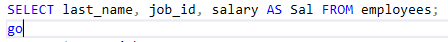
\includegraphics[width=15cm]{./Imagenes/actividad_01_01a} 
	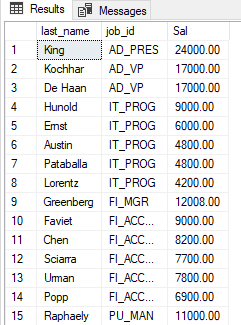
\includegraphics[width=6cm]{./Imagenes/actividad_01_01} 
	\end{center}

	\item SELECT * FROM job\_grades;
	\\Es incorrecta, la sentencia correcta sería:
	\\
	\\SELECT * FROM jobs;
	\begin{center}
	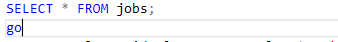
\includegraphics[width=11cm]{./Imagenes/actividad_01_02a} 
	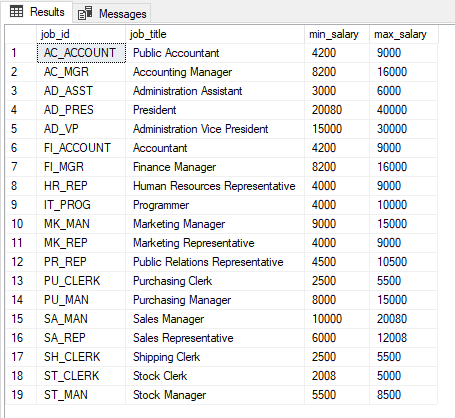
\includegraphics[width=11cm]{./Imagenes/actividad_01_02} 
	\end{center}
	
	\item SELECT employee\_id, last\_name sal x 12 ANNUAL SALARY FROM employees;
	\\Es incorrecta, la sentencia correcta sería:
	\\
	\\SELECT employee\_id, last\_name, salary * 12 'ANNUAL SALARY' FROM employees;
	\begin{center}
	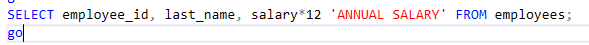
\includegraphics[width=15cm]{./Imagenes/actividad_01_03a} 
	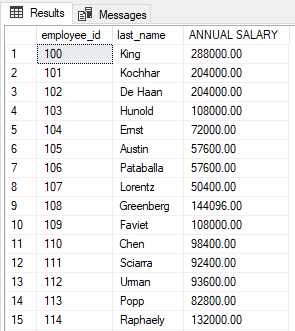
\includegraphics[width=7cm]{./Imagenes/actividad_01_03} 
	\end{center}

\end{itemize} 